\documentclass[12pt,a4paper,openright,twoside]{book}
\usepackage[utf8]{inputenc}
\usepackage{disi-thesis}
\usepackage{code-lstlistings}
\usepackage{notes}
\usepackage{shortcuts}
\usepackage{acronym}
\usepackage[inkscapeformat=png]{svg}

\newcommand{\fonte}[1]{{\color{gray} \small \hypersetup{citecolor=gray} Source: #1}}

\school{\unibo}
\programme{Corso di Laurea Magistrale in Ingegneria e Scienze Informatiche}
\title{A Kotlin Multiplatform implementation of Aggregate Computing based on XC}
\author{Cortecchia Angela}
\date{\today}
\subject{Laboratorio di Sistemi Software}
\supervisor{Prof. Pianini Danilo}
\cosupervisor{Dott. Farabegoli Nicolas}
\session{Quarta}
\academicyear{2022-2023}

%!TeX root = thesis-main.tex
\usepackage{color}

\definecolor{darkgreen}{rgb}{0,0.5,0}
\lstdefinelanguage{kt}{
    frame=single,
    basewidth=0.5em,
    language={kotlin},
    keywordstyle=\color{blue}\textbf,
    commentstyle=\color{darkgreen},
    keywordstyle=[2]\color{cyan},
    keywords=[2]{Aggregate, Field,InboundMessage, OutboundMessage, SingleOutboundMessage,Message,Path,YieldingScope,Network,State,
    AggregateContext,AggregateResult,YieldingContext,YieldingResult},
    keywordstyle=[3]\color{orange},
    keywords=[3]{exchange,exchanging,repeat,repeating,share,sharing,neighboringViaExchange,Collektive,aggregate,yielding},
    keywordstyle=[4]\color{teal}\textbf,
    keywords=[4]{ID,Scalar,Initial,Return,Payload,*,R,X,Init,Ret,Int,Double,Boolean},
    keywordstyle=[5]\color{olive},
    keywords=[5]{read,mapTo,stateAt,messagesAt,newField,excludeSelf,currentPath,mapToConstantField,getPosition,map,distanceTo,hood},
    keywordstyle=[6]\color{blue},
    keywords=[6]{also,it,run,let,context},
    keywordstyle=[7]\color{purple},
    keywords=[7]{neighborCounter,gradient,gradientEntrypoint,distances,distanceBetween,LocalSensing,DistanceSensor,sense,channel,channelWithObstacles},
    keywordstyle=[8]\color{violet},
    keywords=[8]{POSITIVE_INFINITY}
}
\acrodef{iot}[IoT]{Internet of Thing}
\acrodef{dsl}[DSL]{Domain Specific Language}
\acrodef{vm}[VM]{Virtual Machine}
\acrodef{ac}[AC]{Aggregate Computing}
\acrodef{fc}[FC]{Field Calculus}
\acrodef{cps}[CPS]{Cyber-Physical Systems}
\acrodef{cas}[CAS]{Collective Adaptive Systems}
\acrodef{jvm}[JVM]{Java Virtual Machine}
\acrodef{dsl}[DSL]{Domain Specific Language}
\acrodef{ast}[AST]{Abstract Syntax Tree}
\acrodef{ir}[IR]{Intermediate Representation}
\acrodef{ci}[CI]{Continuous Integration}
\acrodef{cd}[CD]{Continuous Deployment}
\acrodef{js}[JS]{JavaScript}
\acrodef{cicd}[CI/CD]{\ac{ci} and \ac{cd}}
\acrodef{kmp}[KMP]{Kotlin Multiplatform}

\mainlinespacing{1.241} % line spacing in mainmatter, comment to default (1)
\begin{document}

\frontmatter\frontispiece

\begin{abstract}
    The integration of technology in everyday activities is rising, with objects being increasingly equipped with
    computational capabilities and interconnected to form the Internet of Things, leading to the need for
    innovative cyber-physical services capable of creating a fast bridge between the real and virtual world.

    The central idea of this thesis focuses on leveraging Kotlin Multiplatform to enhance aggregate computing based on
    XC principles, addressing challenges in devreloping versatile solutions across different environments,
    with the need of efficient and scalable applications operating from cloud to edge to mesh networks.

    This thesis combines theoretical analysis, software development, and performance evaluation to assess
    the effectiveness of the objective, demonstrating versatility and efficiency.
    There is a notable improvement in performance, scalability, and adaptability across in different network environments.
    With the proposed approach, the developed solution appears to be more efficient and effective in addressing
    complex challenges within systems rather than the current state of the art.
    The results demonstrate the transformative potential of this technology, suggesting that it can lead to
    more efficient and versatile service development.

    In summary, this thesis shows the feasibility of using Kotlin Multiplatform to implement aggregate computing
    based on XC, demonstrating that the proposed approach is more efficient and scalable than the state of the art.
    Improved performance and scalability are emphasised through this approach, which opens doors for more efficient and
    adaptable solutions.
    Future exploration and improvement of this technology has the potential to advance interconnected systems and innovations.
    This study sets the stage for future developments that could improve service efficiency and effectiveness.
\end{abstract}

\begin{dedication} % this is optional
To my family, a constant source of support,\\
who has always allowed me to choose\\ my own path with freedom and trust.
\end{dedication}

%----------------------------------------------------------------------------------------
\tableofcontents   
\listoffigures     % (optional) comment if empty
\lstlistoflistings % (optional) comment if empty
%----------------------------------------------------------------------------------------

\mainmatter

%! Author = angela
%! Date = 24/01/24
% !TeX root = ../thesis-main.tex

%----------------------------------------------------------------------------------------
\chapter{Introduction}
\label{ch:introduction}
%----------------------------------------------------------------------------------------
This chapter introduces the background of this thesis, including our position, main objectives,
and the current state of the art.

\section{Context}
\label{sec:context}

Computing devices are becoming cheaper and more \emph{ubiquitous}, increasing the complexity of distributed systems.
It is now common for individuals to own multiple computing devices of varying types,
resulting in technology becoming more integrated into daily activities.
Hence, the need to engineer and coordinate the operations in such systems, one way is to program and operate in terms of
    \emph{aggregates} of devices, rather than manage each single device.
In fact, the coordination of macroscopic behaviour in collective systems through a single program is a form of
~\emph{macroprogramming}.
However, this approach presents some primary challenges such as ensuring resilience, efficiency and privacy.

\paragraph{Macroprogramming}
The term \emph{macroprogramming} ~\cite{10.1145/3579353} refers to the concept of expressing the macroscopic behaviour of a system through a single
program, usually leveraging macro-level abstractions.
This paradigm is driven by the need to capture \emph{system-level behaviour} while abstracting the behaviour and interaction
of the individual components involved.
Macroprogramming approaches have been suggested to simplify the development of systems involving numerous interconnected
sensors, actuators, and smart devices; they can be applied in contexts like \ac{iot} and \ac{cps}.

By declaring tasks within a specific spatio-temporal region, systems can self-organise and effectively perform the task
at hand, allowing for dynamic adaptation to the current deployment and spatial positions of the components involved.

Macroprogramming abstractions can promote collective behaviour properties, such as self-organising or self-configuring in
the context of \ac{cas}.

\paragraph{Self-Organisation}
Coordination modes are based on the notion that interactions among multiple independent and autonomous software systems
can be designed as a space orthogonal to pure computation.
This idea can be reified into a concept of shared data space, enabling so-called \emph{generative communication}.

Over the course of time, different approaches have been created, such as \emph{Linda} ~\cite{10.1145/2363.2433} and \emph{Mars} ~\cite{865084},
suggesting innovative techniques for programming systems with devices of different nature focusing on the coordination
of centralised local components, but not on the distribution of the systems.
The main problems that can be encountered in distributed systems are dealing with
    \emph{(i)} openness, as unexpected environment changes,
    \emph{(ii)} large scale of agents and coordination abstractions to be managed,
    \emph{(iii)} intrinsic adaptiveness, such as the ability to intercept relevant events and react to them, guaranteeing
        the resilience of the system.

The challenges necessitate a \emph{self-organising coordination} approach, wherein coordination abstractions solely
manage logical interactions.
This ensures the emergence of global and robust patterns of correct coordination behaviour.


\subsection{Computational Fields}
\label{subsec:computational-fields}

\paragraph{Field-Based Coordination}
To facilitate self-organisation patterns of agents in complex environments, the concept of \emph{coordination field}
has been introduced.
This abstraction serves as a navigational tool for agents over the actual environment.

In this context, the tuple-based middleware \emph{TOTA} (Tuples On The Air) ~\cite{10.1145/1538942.1538945}
has been suggested to support field-based coordination for pervasive-computing applications.
Initially, each field of the tuple in the system was assigned a name, along with a formula that supports the
if-then-else construct and includes arithmetic and boolean operators to specify the field's behaviour over time.
Secondly, it was introduced an operator in the tuple space responsible for applying formulas using contextual information.\\

Somewhat independently of the challenge of identifying appropriate coordination models for distributed and situated systems,
several studies have tackled analogous issues in the broader endeavour of constructing distributed intelligent systems.
This involves promoting higher abstractions of spatial collective adaptive systems.

\paragraph{Field Calculus}
Among the studies such as for managing space-time computing models for the manipulation of distributed data structures,
the notion of \emph{computational fields} were proposed ~\cite{VIROLI2019100486}.
Consequently, the ~\ac{fc} has been proposed as a foundational model for the coordination of computational
devices spread in physical environments, also known as \emph{aggregate computing}.

~\ac{fc} was introduced as minimal core calculus with the aim of capturing the fundaments that make use of computational
fields: functions over and with fields, their evolution over time and the construction of field of values from neighbours.

The main concept of \ac{fc} is to specify the aggregate system behaviour of a network of devices, where devices that can
directly communicate with each other are indicated through a dynamic network relation.
An example of its application is within a sensor network with a range of a broadcast communication.

The behaviour is applied through a functional composition of operators that manipulate the computational fields,
called specification, that can be interpreted locally or globally.
A local specification can describe a computation on an individual device executed in asynchronous ``computation rounds'',
including sending or receiving messages from neighbours, getting information from sensors and computing the local value of the field.
In the global view, a field calculus expression specifies a mapping associating each computation round of each device to
the value that it assumes at that space-time event.

This dual nature inherently facilitates the alignment of individual device behaviour with the overarching global behaviour
of the entire network of devices.

\paragraph{Syntax of field calculus}
\label{par:syntax-of-field-calculus}

\begin{figure}
    \begin{align*}
        \boxed{
            \begin{aligned}
                \q{P} &::= \q{F}\ \q{e} && \text{program} \\
                \q{F} &::= \q{def} \, \q{f(}\bar{\q{x}}\q{)} \{\q{e}\} && \text{function declaration} \\
                \q{e} &::= \q{x} \ | \ \q{v} \ | \ \q{f(}\bar{\q{e}}\q{)} \ | \ \q{if}(\q{e})\{\q{e}\}\{\q{e}\} \ | \ \q{nbr}\{\q{e}\} \ | \ \q{rep}(\q{e})\{(\q{x}) \rightarrow \q{e}\} && \text{expression} \\
                \q{f} &::= \q{d} \ | \ \q{b} && \text{function name} \\
                \q{v} &::= \q{l} \ | \ \phi && \text{value} \\
                \q{l} &::= \q{c(}\bar{\q{l}}\q{)} && \text{local value} \\
                \phi &::= \bar{\delta} \mapsto \bar{\q{l}} && \text{neighbouring field value}
            \end{aligned}
        }
    \end{align*}
    \caption{Field Calculus abstract syntax extracted from~\cite{10.1145/3177774}.}
    \label{fig:field-calculus-abstract-syntax}
\end{figure}
\label{sec:field-based-programming-model}

The \emph{field calculus} is based on a minimal set of operators, in \Cref{fig:field-calculus-abstract-syntax} it is
described its abstract syntax.
\begin{itemize}
    \item \emph{Stateful field evolution}: the expression $rep(e_1)\{(x) \rightarrow e_2\}$ describes a field evolving in time.
        $e_1$ represents the initial field value, the function $(x) \rightarrow e_2$ declares how the field changes
        at each execution;
    \item \emph{Neighbour interaction}: the expression $nbr\{e\}$ builds a neighbouring field, a view of the field
        values in the surroundings of each device where neighbours are mapped to their evaluations of \texttt{e};
    \item \emph{Domain partitioning}: the expression $if(e_0)\ \{e_1\}\ \{e_2\}$ splits the computational field into
        two non-communicating zones hosting isolated computations: $e_1$ where  $e_0$ is \texttt{true} and
        $e_2$ where  $e_0$ is \texttt{false}
\end{itemize}

It was soon proposed an apparently straight-forward combination of state evolution with \texttt{nbr} and sharing with \texttt{rep},
but it turned out that it contained a hidden delay, identified and explained in \cite{fieldc}.
To overcome the problem in the interaction between the two constructs, it has been proposed a new one:
$share(e_1)\{(x) \rightarrow e_2\}$.
This construct differs from \texttt{rep} in the way that the variable \texttt{x} is interpreted ad each round, that is
identified as a \emph{neighbouring field} rather than a value.
In this case, $e_2$ is responsible for processing the neighbouring field into a local value shared with the
neighbours at the end of the evaluation.
Therefore, the \texttt{share} improves the communication speed.

\subsection{Aggregate Computing}
\label{subsec:aggregate-computing}

\paragraph{Aggregate programming}
Aggregate programming elaborates a layered architecture that aims to simplify the design, creation and maintenance of
distributed systems \cite{CASADEI2019252}.

Through this methodology, the fundamental unit of computation shifts from an individual device to a collaborative
ensemble of devices.
It elaborates a layered architecture that aims to simplify the design, creation and maintenance of complex distributed
systems.

Moreover, aggregate programming provides mechanisms for robust and adaptive coordination through simple programming APIs
that implicitly guarantee safety and resilience.
This framework is useful in large-scale scenarios, where there is insufficient fixed network infrastructure, as seen in
situations like crowd management during large public events.

In various environments, interactions between wearable devices such as smartphones can support different kinds of services,
including crowd detection, crowd-aware navigation or dispersal advice.

\paragraph{Aggregate computing}
~\ac{ac} is a paradigm and engineering approach for the compositional development of self-adaptive ~\ac{iot} services
from a global perspective ~\cite{10.1145/3579353}.

It has been developed with the core idea of functionality composing collective behaviours to achieve effective and resilient
complex behaviours in dynamic networks.
It views a given environment as a whole programmable entity whose parts collaboratively produce and consume services
across space and time.
~\ac{ac} is based on the principles of~\ac{fc} that is a functional programming model used to specify
and compose collective behaviours with formally equivalent local and aggregate semantics.

The concept of \emph{computational fields} can be viewed as a distributed data structure,
with the aim of conceptually mapping each device to a value produced in a program, considering both
space and time.
Therefore, its structure supports the specification, analysis, simulation and runtime execution of \emph{collective}
or \emph{aggregate} services, independently of the specific~\ac{iot} architecture.

This paradigm has three key traits that characterise it:
    \emph{(i)} \emph{Global stance with global-to-local mapping}, where the target of system design is the entire distributed
        \ac{iot} ecosystem,
    \emph{(ii)} \emph{Behaviour compositionality}, whereby a rich collective service can be described in terms of the functional
        composition of simpler collective services, and
    \emph{(iii)} \emph{Abstraction}, by which aggregate services enable adaptivity at different levels by abstracting from low-level
        issues and details.
These attributes are crucial both in the design phase, where intricate solutions can frequently be articulated concisely
and declaratively, and in the operational phase, where considerable flexibility is granted to the devops team and the
platform regarding execution specifics and deployment strategies.


\begin{figure}
    \centering
    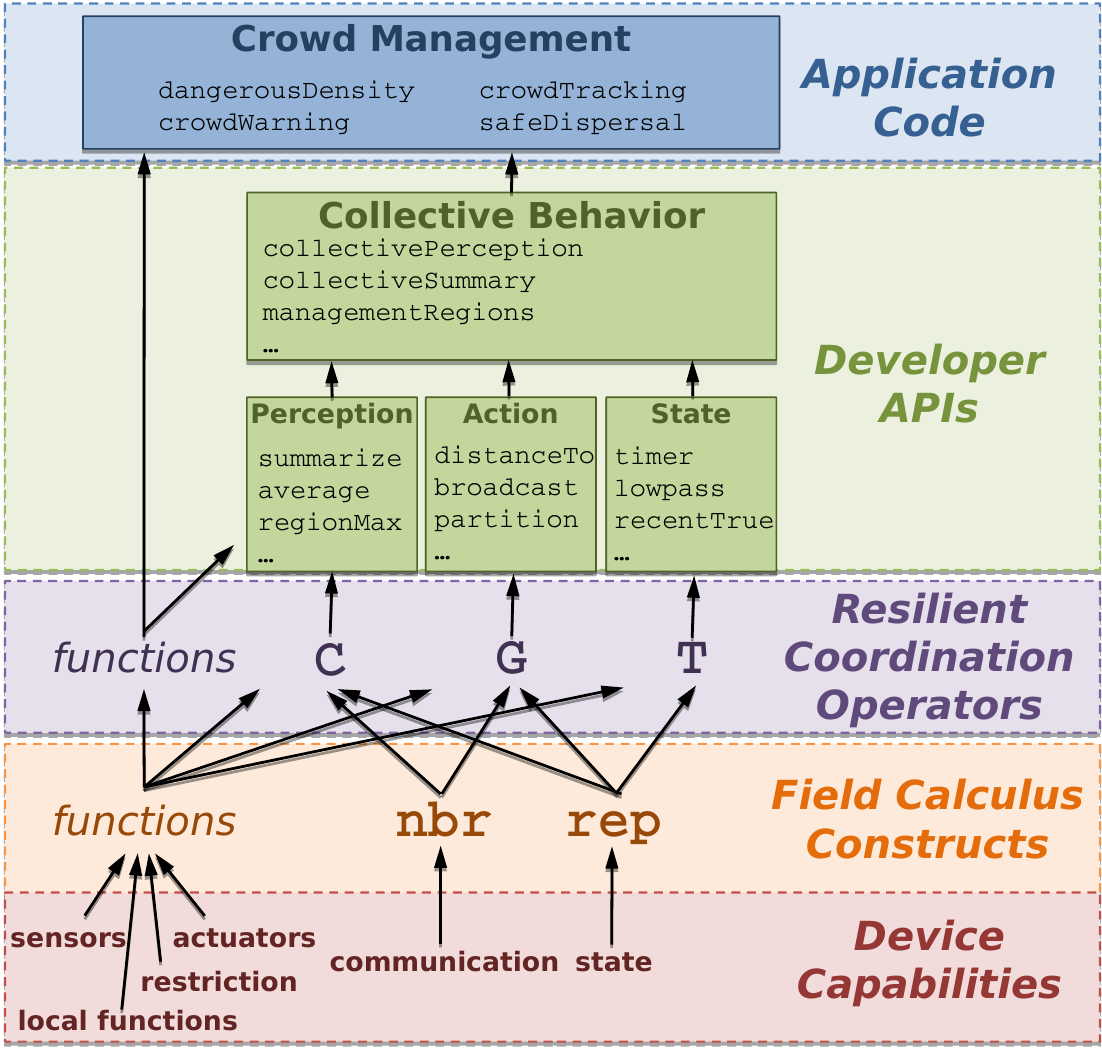
\includegraphics[width=.7\linewidth]{figures/aggregate-programming-stack}
    \caption{The aggregrete programming stack \cite{7274429}.}
    \label{fig:ac-stack}
\end{figure}
%todo cite figure

\paragraph{Software platforms}
~\ac{ac} is designed to address many application scenarios, typically characterised by inherent distribution, heterogeneity,
mobility and a lack of stable infrastructure.
There are various strategies by which an~\ac{ac} system can run, contingent upon the selected and implemented
communication methodologies.

Programs can be executed within a fully distributed peer-to-peer environment, where end devices communicate directly
with peer neighbours, and each independently runs its fragment of aggregate logic.

On the opposite side, there are entirely centralised solutions, where end devices function solely as manager for sensors
and actuators, forwarding perceptions upstream to one or more servers.
These servers perform computations on behalf of the devices and subsequently transmit actuation data downstream.
Thanks to this flexibility of its applications,~\ac{ac} has the potential to facilitate the creation of a more systematic
spectrum for transitioning between cloud and distributed systems.
This approach also embraces the emerging domains of Edge ~\cite{8795355} and Fog Computing ~\cite{bdcc2020010}.

\paragraph{Aggregate computing in adaptive \ac{iot} Services}
Thanks to its features, \emph{aggregate computing} is well suited for the development of \emph{Opportunistic \ac{iot}
Services}, supporting the properties:
\begin{itemize}
    \item \emph{Dynamicity}: the direct support for opportunistic service activation and evolution is achieved through
        code mobility and constructs that define dynamic domains of computations dependent on space and time;
    \item \emph{Context-awareness}: aggregate programs utilize sensors, communication driven by neighborhood interactions,
        and iterative execution to consistently evolve the set of local contexts.
        This evolution forms the basis for the unfolding of computation and coordination logic;
    \item \emph{Co-location}: as a natural method to define the concept of neighbourhood, relies on a physical space basis.
        \ac{ac} inherently incorporates locality (both in space/time and purpose) to organise interactions and activities;
    \item \emph{Transience}: \ac{ac} provides constructs that directly supports the execution of distributed services
        based on time and context awareness.
\end{itemize}

\paragraph{Computational model}
%todo I can see this as ubiquitous language
There are some concepts and relationships included in the \emph{aggregate computing} context:
\begin{itemize}
    \item \emph{Aggregate program}: an executable representation of specific aggregate logic that defines a collective behaviour;
    \item \emph{Aggregate system}: a set of interconnected nodes or devices that support the collective execution of aggregate programs;
    \item \emph{Aggregate application}: a specific aggregate logic operating on a designated aggregate system, aimed at
        solving particular problems in a specific context;
    \item \emph{Node}: also referred to as \emph{device}, it represents an individual \ac{ac}-enabled entity, potentially
        equipped with sensors and actuators;
    \item \emph{Neighbourhood}: the logical or physical set of nodes that can be directly contacted by a given node;
    \item \emph{Global or local sensor}: a source for global or local information;
    \item \emph{Global or local actuator}: a global or local actionable device for environment-directed actions;
    \item \emph{Global or local computational environment}: anything that is detectable and subject to action through the
        use of global (or local) sensors and actuators
        This also includes the shared functionalities offered by the platform.
\end{itemize}

The networked devices inside an aggregate system compute and communicate at asynchronous rounds of execution.
Each round, each device executes the global aggregate program according to the local semantics; then it updates its internal
state and lastly generates the data for the external communication.

The round is performed by taking into account the computational context created by the previous state, sensor data and
messages from neighbouring devices.
After the execution of the round, result data are made available to neighbours and eventually instructed actuations are
locally executed.
The system can continuously react to changes by repeatedly executing rounds, allowing for self-adaptation to contextual changes.

\paragraph{Models alignment}
Due to the high-level and platform-independent metamodels of \ac{iot} and \ac{ac} systems, each with different goals or
abstraction levels, it is necessary to align the two metamodels.
This ensures that their unique focus is taken into account.

There are some main differences between the two metamodels:
\begin{itemize}
    \item the concept of device is different, for \ac{ac} is logical and is not the same as a device component of a Smart Object;
    \item although ensembles of Smart Objects are conceptualised as firs-class concept in \ac{ac}, they are not explicitly
        represented in the \ac{iot} system metamodel;
    \item the concept of neighbourhood in \ac{ac} regulates local, contextual communication among its devices.
        However, this concept cannot be explicitly mapped to \ac{iot} system concepts because device-to-device relationships
        are abstracted away from the metamodel.
\end{itemize}

\subsection{XC}
\label{subsec:xc}
\xc{} is an experimental programming language design to develop \emph{homogeneous} distributed systems.
Those kinds of systems consist of similar devices that communicate to neighbours and execute the same program.
The aim of this experimental language is to push the abstraction boundaries farther than actual existing approaches.

Many issues can arise in distributed systems, like concurrency, remote communication, asynchronous execution, message
loss, and device failures.
These kinds of problems must be taken into account when designing a programming language for such systems.
Some of the possible applications of this approach may be crowd management, gossip-based data aggregation, task allocation
in robot swarms and coordination of enterprise servers. %todo add cites that are in the xc paper

The homogeneity in large-scale systems also arises when each device executes a program from a predefined set, reflecting
a homogeneous configuration featuring a single program with an initial branch.

%This design eliminates the need to handle the aforementioned problems explicitly.
%Additionally, distributed programs with independent devices retain composability through a mechanism called \emph{alignment}.

\paragraph{System model}
Devices that can send or receive messages are called \emph{neighbours}, and they can change dynamically to model network
delays, failures or spatial movements.

Based on existing homogeneous systems, the device behaviour has been abstracted through a notion of \emph{execution round},
in which a device independently executes an \xc{} program and sends the resulting messages to its neighbours.
Referring to \emph{macroprogramming}, each device's behaviour in the network is developed as a single program, with no
assumption of when an execution round will occur, meaning that they are entirely asynchronous.

Messages are handled queueing up in a buffer; when a device executes its \xc{} program, it processes the received
messages producing others to send to neighbours, that in turn will process their messages.
%todo insert graph of the system model

It can occur that a device executes multiple rounds before a neighbour executes its own, in that case the neighbour will
only see the last received message from the first device; newly received messages will overwrite the older ones.
Messages can persist across rounds; they are not removed from the buffer after they have been read unless they expire.
The devices for which a message is available in a certain round are considered the \emph{neighbours} for that round.

\paragraph{Data types}
\xc{} features two kinds of values:
    \emph{(i)} \emph{local values (l)}, that include traditional types, and
    \emph{(ii)} \emph{neighbouring values (nvalues)}, a map from the device identifier to their local values, used to describe
        the set of values received from and sent to neighbours.
In highly decoupled networks, it can occur that not all devices will produce a value, for this reason it will be used
a default value.

Different types of operations can be applied to \emph{nvalues}, where the function passed is repeatedly applied to
neighbour's values in a field $\underline{w}$, excluding the self-value.
A \emph{local value} can be also converted to a \emph{nvalue} using the default value for every device.

\paragraph{Communication in XC}
\label{par:communication-in-xc}

\xc{} is based on a key communication primitive:\\ $exchange(e_i,\ (\underline{n}) \rightarrow \ \texttt{return} \ e_r \ \texttt{send} \ e_s)$
which is evaluated as follows.
    \emph{(i)} the device computes the local value from the initial value $e_i$.
    \emph{(ii)} the variable $\underline{n}$ gets substituted with the computed nvalues $\underline{w}$ of the received messages, eventually
        using the local value as default, the exchange returns the computed value $v_r$ from $e_r$.
    \emph{(iii)} $e_s$ evaluates to a nvalue $\underline{w}_s$ consisting of local values to be sent to neighbours,
        that will take their corresponding value from $\underline{w}_s$ and use it for the execution of their next round.

A common pattern that can be used is to access neighbour's values through the use of the \texttt{exchange} function, as follows.\\
$nbr(e_i,\ e_s) = exchange(e_i, (\underline{n}) \rightarrow \texttt{return} \ \underline{n} \ \texttt{send} \ e_s)$,
which means that the value of expression $e_s$ is sent to neighbours and returns the received values gathered as
$\underline{n}$ with its default, thus providing a view on neighbours' values $e_s$.
Often the expressions $e_r$ and $e_s$ coincide, in this case, the \texttt{exchange} function is
$exchange(e_i, (\underline{n}) \rightarrow \texttt{retsend} \ e)$.

The crucial aspect of the \xc{} expressivity is that \texttt{exchange} can send a different value to each neighbour,
allowing custom interaction through them.

\paragraph{Alignment}
An aggregate program has the capability to execute multiple exchange-expressions.
In order to guarantee the dispatching of messages to corresponding expressions throughout different rounds,
    \xc{} introduces the concept of \emph{alignment}.
The \emph{alignment} is a mechanism that enables developers to abstract over asynchronous execution while still retaining
composability.
In this way, \xc{} guarantees that the values produced by an exchange are processed by the corresponding function
in the next round.
To accomplish this, it verifies whether it's in the same position of the Abstract Syntax Tree (AST) and of the stack frame.

\paragraph{Conditionals}
\xc{} supports conditional expressions, like $if\ (cond)\ \{e_1\}\ else\ \{e_2\}$.
An exchange aligns only across the devices that take the same branch; thus, it evaluates only aligned sub-expressions.
This means that a network can be split by a conditional expression into two non-communicating subnetworks, each
evaluating a different branch without cross-communication.

\paragraph{Fault tolerance}
\xc{} programs are resilient to failures: in case a node gets disconnected or messages get lost, the failed node won't
show up among the neighbours of a given node in the next alignment.
The logic of \emph{exchange} is set to let neighbours' messages collectively operate, in order to make no assumptions
on their number or identity.
It is crucial to highlight that XC does not inherently offer assurances regarding fault tolerance.
As a Turing-complete language, the capability to program non-resilient behaviour is inevitably present.

\section{Motivations}
\label{sec:motivations}
%vantaggi > benefits/utility

In this section, the motivations for developing a new programming language for aggregate computing will be illustrated,
the objectives that are intended to be achieved and the benefits that are expected to be obtained.

From an engineering perspective, the construction of \ac{iot} applications differs substantially from that of traditional
software, especially when a particular service, to be realised, requires the coordination of devices of different nature.

\paragraph{Challenges and innovations}
Over the course of time, different approaches have been proposed to program these systems, such as TOTA, SAPERE, Aggregate
Computing, Linda, MARS and others. %todo cite them

The most successful solution at the moment involves the use of Cloud Computing (see ~\Cref{fig:cloud-edge-continuum}),
which provides virtualised resources on a large scale, but presents limitations in terms of latency (due to the physical
distance between machines) and scalability (due to centralisation).

For this reason, Edge Computing and Fog Computing have recently emerged, aiming to bring resources closer to the outer
edge of the network, where interoperability problems between devices and complexity in managing distributed resources increase.

The design of applications capable of operating indistinctly on the cloud, on the edge, or even on a mesh network
(in fact, on a computational continuum that goes from the edge to the cloud) can benefit from unconventional approaches,
such as Aggregate Computing.

\begin{figure}
    \centering
    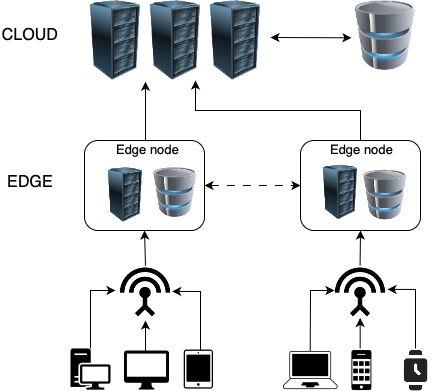
\includegraphics[width=.5\linewidth]{figures/edgecloud}
    \caption{This figure shows the continuum of computing from the edge to the cloud, highliting the edge-cloud verticality
    and the heterogeneity of devices.}
    \label{fig:cloud-edge-continuum}
\end{figure}

\subsection{Heterogeneity limitations}
\label{subsec:heterogeneity-limitations}

One of the limitations of current collective programming approaches is the management of heterogeneity.
In fact, the system assumes that there is a certain uniformity of capabilities along the continuum, or that it is possible
to abstract it in some way (see, for example, the ``pulverization'' approach ~\cite{fi12110203}).

However, when the system includes devices whose nature is profoundly different (imagine, for example, a system where both
well-equipped servers and tiny wearable or implanted devices with very moderate computing capabilities participate, as
shown in ~\Cref{fig:smart-network-objects}), finer mechanisms are needed.
A somewhat analogous problem appears in functional programming when modelling effects, and recent proposals aim to capture
them in the form of capabilities.

\begin{figure} %[!ht]
    \centering
    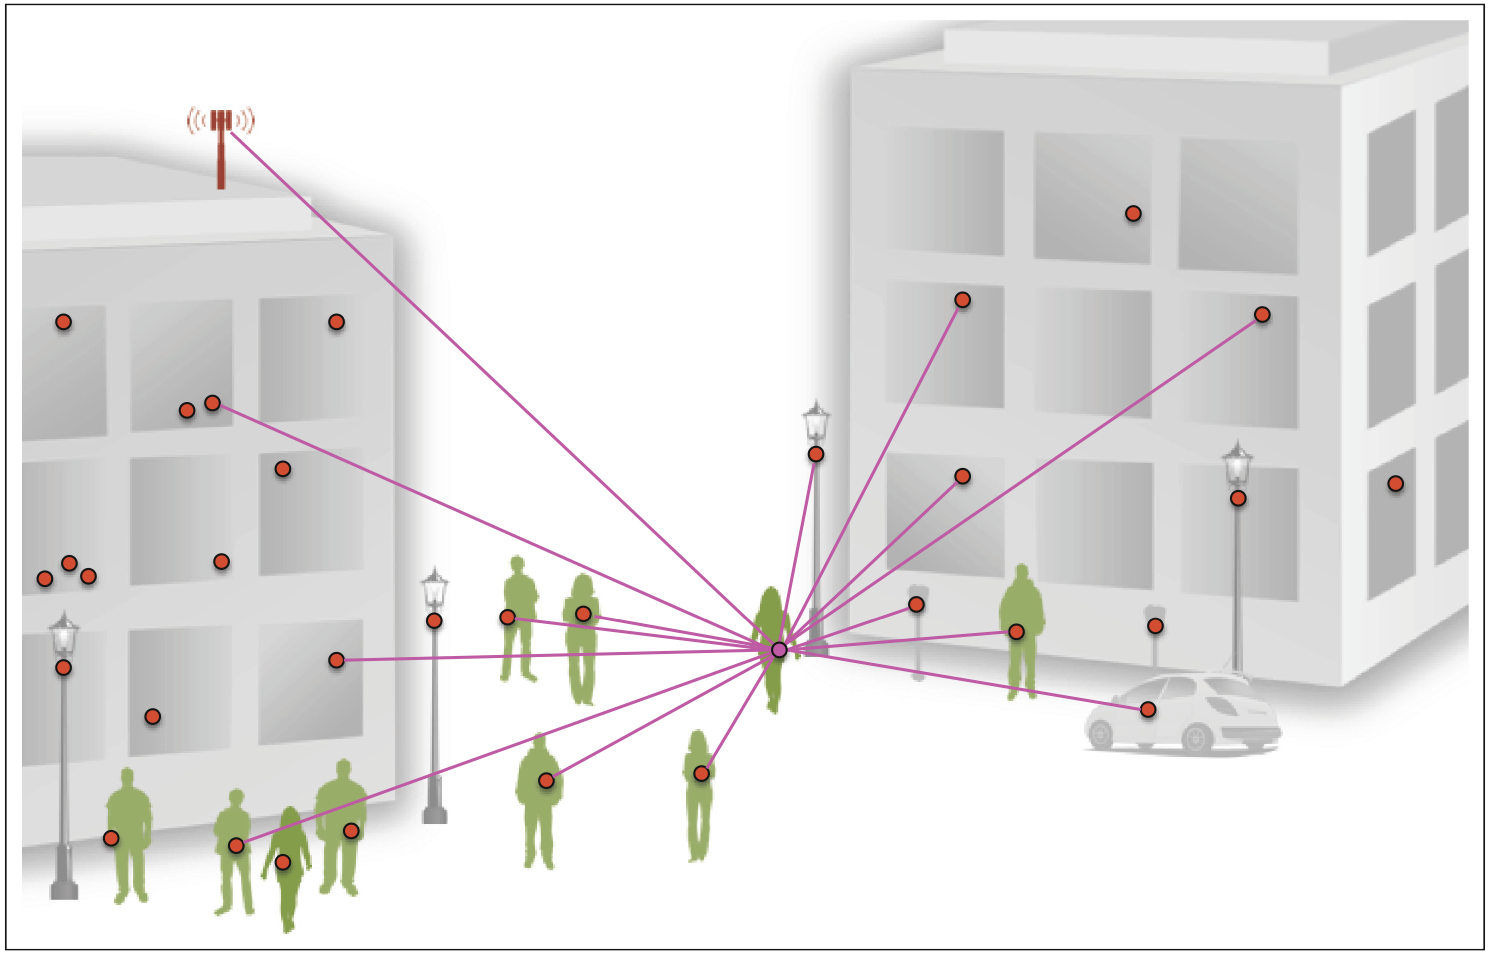
\includegraphics[width=.8\linewidth]{figures/smart_network_objects}
    \caption{Our world is increasingly populated with a wide range of computing devices, embedded in our environment
    and with many opportunities for local and even location-indipendent interactions on fixed network infrastructures.}
    \label{fig:smart-network-objects}
\end{figure}

\subsection{Goal}
\label{subsec:goal}

%lo scopo di questa tesi è quello di estendere il DSL gia esistente 'Collektive', applicando i concetti di XC
%ai costrutti di programmazione aggregata, cercando così di migliorarne le performance in modo tale da
%rendere questo dsl competitivo nei confronti degli approcci gia esistenti

%inoltre si vuole creare un incarnazione di questo DSL in maniera tale da poter eseguire simulazioni attraverso
%il simulatore Alchemist.

%todo speak about performances increase

The goal of this thesis is to extend the existing \ac{dsl} \emph{Collektive} by applying the concepts of \xc{} to
aggregate programming constructs, thus seeking to improve its performance in order to make this \ac{dsl} competitive
against existing approaches.
Furthermore, the aim is to create an incarnation of this \ac{dsl} in such a way that it can execute simulations through
the Alchemist simulator.

It is necessary to rely on technologies and languages that can run on any device.
Kotlin Multiplatform will be used, which allows developers to write code that can be compiled for multiple targets,
including JVM (ideal for server environments), Javascript (browser), Android, iOS (including watchOS and tvOS), and native versions
(for Windows, MacOS, and Linux, both for x86 and ARM CPUs).

%todo cite those things up there

\paragraph{Impact}
The development of a new programming language for aggregate computing will have a significant impact on the development
of distributed systems, especially in the \ac{iot} and \ac{cps} domains.
The new language will allow developers to write programs that can be executed on any device, regardless of its nature,
and will be able to communicate with other devices in the network, thus simplifying the development of complex systems.

%todo add more??

\section{State of Art}
\label{sec:state-of-art}

In this section, it will be presented the state of the art in the field of aggregate computing, focusing on the main existing
frameworks and languages and their limitations.

Still, in terms of portability to heterogeneous systems, there are currently several software programs that implement the
semantics of aggregate programming derived from field calculus, but they are not interoperable with each other.

\subsection{ScaFi}
\label{subsec:scafi}

\emph{ScaFi (Scala Field)} is a Scala-based framework for aggregate programming\\ ~\cite{CASADEI2022101248}.
It provides a \emph{\ac{dsl}}, libraries, a simulation environment with a GUI, integrated with the
Alchemist simulator ~\cite{10.1007/978-3-030-78198-9_10}, and an actor-based runtime for the development of aggregate computing-based systems.
\emph{ScaFi}'s core is based on a variant of the \emph{field calculus} called \emph{F ScaFi} ~\cite{10.1007/978-3-030-61470-6_21},
which peculiarity is to handle standard values to provide a simplified setting for \ac{dsl} embedding.

This is achieved by introducing a notion of ``computation against neighbours'', meaning that is a computation whose
output depends on the most recent values received from neighbours.

\begin{figure}
    \centering
    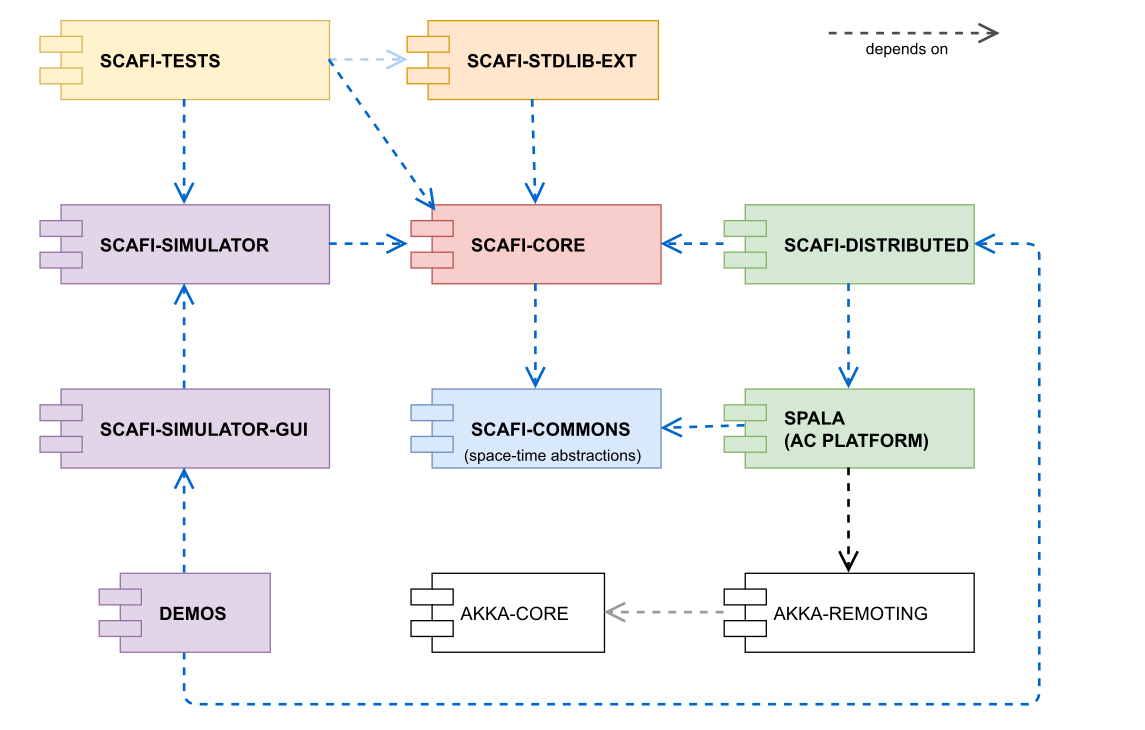
\includegraphics[width=.7\linewidth]{figures/scafi_structure}
    \caption{High-level architecture of the ScaFi toolkit.}
    \label{fig:scafi-structure}
\end{figure}

The architecture of \emph{ScaFi} consists of various modules, as seen in ~\Cref{fig:scafi-structure}.
The \ac{dsl} and standard library of reusable functions are implemented in the \texttt{scafi-
core} module; meanwhile, the modules \texttt{scafi-simulator} and \texttt{scafi-simulator-
gui} provide a simulation
environment of aggregate systems with a graphical user interface.

The main applications of \emph{ScaFi} are in the development of swarm systems ~\cite{10336236}, crowd management, wireless sensor network (WSN) ~\cite{9935036}
and smart city applications.

\emph{ScaFi} is capable of running aggregate programs on the \ac{jvm} and also on web browser thanks
to the \emph{ScaFi Web} tool ~\cite{10.1007/978-3-030-78142-2_18}, which allows the rapid prototyping of aggregate programs.
On the other hand, it does not provide an aggregate standard library in the public version, neither supports to
different advanced mechanisms.
Furthermore, it is based on Scala 2, which means that it needs a review to be updated to Scala 3.

Since \emph{ScaFi} only supports \ac{jvm} and web-based applications, it is not well-suited for the development of complex distributed systems.
devices and communication technologies, such as thin devices that do not support \ac{jvm}, which limits the heterogeneity of
devices that can be used in the system.

\subsection{Protelis}
\label{subsec:protelis}
%todo cite Java. xtext,
\emph{Protelis} ~\cite{protelis} is a functional programming language that implements a higher-order version of the \emph{field calculus},
exposed through a C-like syntax, enabling the construction of widely reusable components of aggregate systems.
It also provides various domain-specific APIs that are interoperable with Java.
\emph{Protelis} has been developed since no foundational API for resilient, situated and distributed systems can be found
in the Java ecosystem.
It offers an implementation for the interoperability with the \emph{Alchemist} simulator, where it can be seen its
practical use in the development of aggregate systems.

\begin{figure}
    \centering
    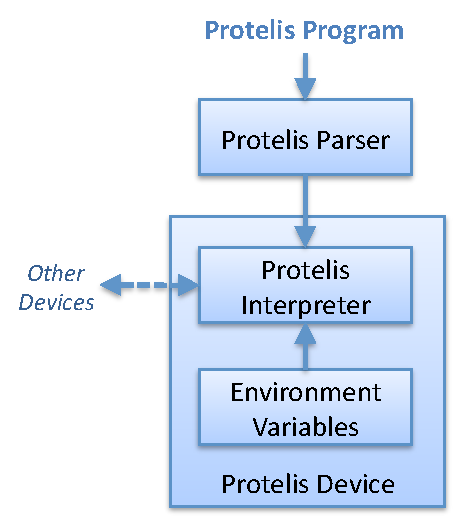
\includegraphics[width=.5\linewidth]{figures/protelis-structure}
    \caption{The abstract architecture of Protelis.}
    \label{fig:protelis-structure}
\end{figure}

As seen in the \emph{Protelis} architecture (~\Cref{fig:protelis-structure}), an interpreter executes a pre-parsed program at regular intervals,
that communicates with other devices and draws contextual information from the environment.
This is instantiated by specifying when the executions occur, how the devices communicate and how the environment is
represented.

A key reason for this choice is that Java is highly portable across systems and devices.
Another important reason is that Java's reflection mechanisms make it easy to import a large number of useful libraries
and APIs for use in Protelis.

It is based on \emph{Xtext}, a framework for the development of domain-specific languages, which provides a set of tools
and libraries for the development.
For this reason necessary requires a \ac{jvm} to run, which limits the heterogeneity of devices
that can be used in the system.

\subsection{FCPP}
\label{subsec:fcpp}
\emph{FCPP} ~\cite{9196401} is an implementation of the \emph{Field Calculus} as a C++ library, with tools for simulations of distributed systems.
This library is built as a component-based system ~\Cref{fig:fcpp-structure}, with the aim of being easily extensible and reusable in different contexts.

It has a performance-oriented implementation based on compile-time optimisations, and it is designed to support
simulated systems executed in parallel or self-organising cloud application.

\begin{figure}
    \centering
    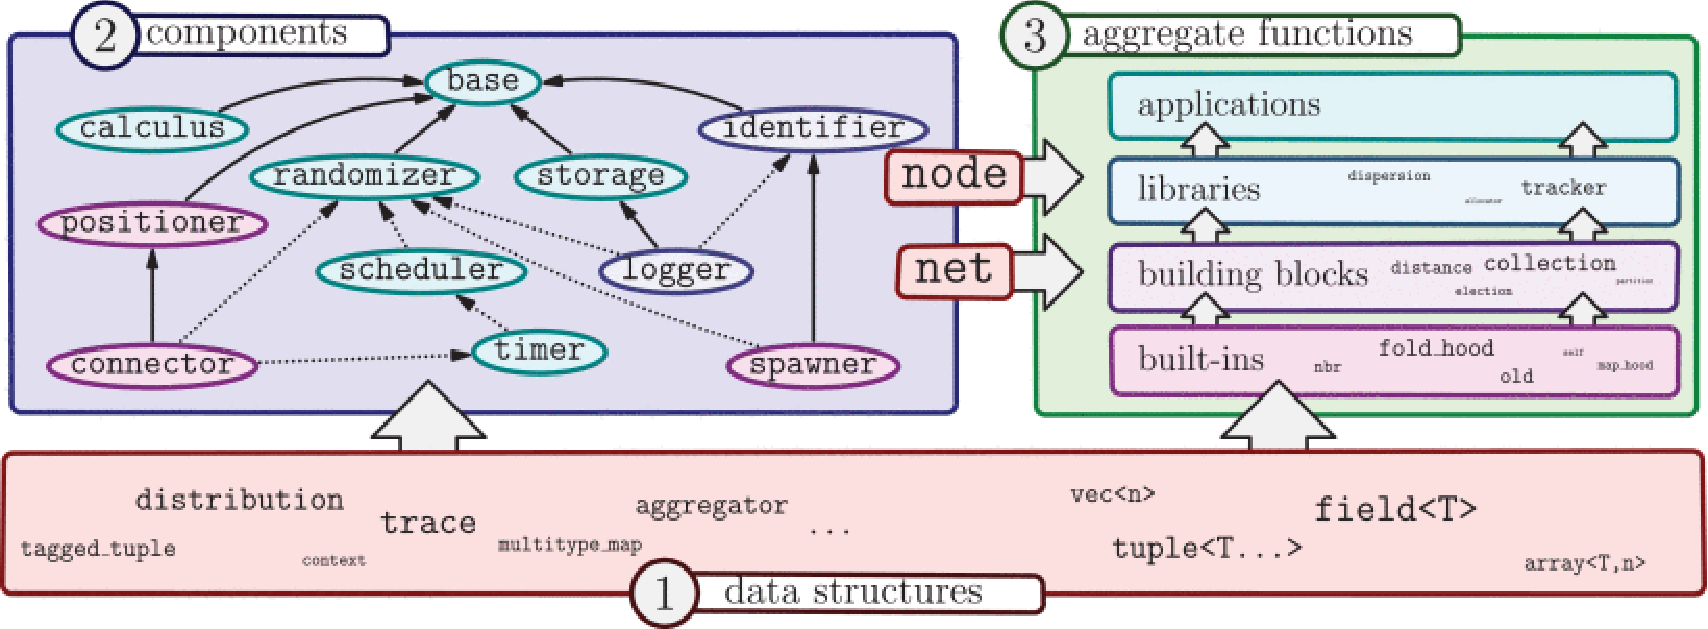
\includegraphics[width=.8\linewidth]{figures/fcpp-structure}
    \caption{The Software architecture of FCPP represented as three main layers.}
    \label{fig:fcpp-structure}
\end{figure}

Being implemented in C++, allows \emph{FCPP} to be used in a wide range of devices, including embedded systems and
microcontrollers, for which a C++ compiler is available.
Although \emph{FCPP} is designed as a flexible and easily extensible platform, its currently supported range of features
is more limited than \emph{Alchemist}'s.

It allows running aggregate programs on low computational capacity devices.
However, its syntax is less ergonomic compared to other languages, making it unlikely to reach a mainstream developer audience.

\paragraph{Final considerations}
Those three illustrated frameworks have more or less the same expressive power, with few notable differences.
The main differences among them are between \emph{ScaFi} and \emph{FCPP}, that are \emph{internal} \ac{dsl} implemented in Scala
and C++, and \emph{Protelis} that is an \emph{external} \emph{dsl}, interpreted in the \ac{jvm}.

Considering their syntax, \emph{ScaFi} and \emph{Protelis} partially imitate the abstraction level of the \emph{field calculus},
being bound by the specific syntactic constraints of their host languages.
Whereas, \emph{Protelis}' syntax is more neat and specifically designed for field computation.

However, the more complex syntax of \emph{Scafi} and \emph{FCPP} may prove easier to learn for programmers already familiar with Scala and C++.
%! Author = angela
%! Date = 24/01/24
% !TeX root = ../thesis-main.tex
\definecolor{ddarkgreen}{rgb}{0,0.5,0}
\lstdefinelanguage{kt}{
    frame=single,
    basewidth=0.5em,
    language={kotlin},
    keywordstyle=\color{blue}\textbf,
    commentstyle=\color{ddarkgreen},
    keywordstyle=[2]\color{cyan},
    keywords=[2]{Aggregate, Field,InboundMessage, OutboundMessage, SingleOutboundMessage,Message,Path,YieldingScope,Network,State,
        AggregateContext,AggregateResult,YieldingContext,YieldingResult},
    keywordstyle=[3]\color{orange},
    keywords=[3]{exchange,exchanging,repeat,repeating,share,sharing,neighboringViaExchange,Collektive,aggregate,yielding},
    keywordstyle=[4]\color{teal}\textbf,
    keywords=[4]{ID,Scalar,Initial,Return,Payload,*,R,X},
}

\chapter{Contributions}
\label{ch:contributions}
In this chapter, will be presented the main contributions of this thesis.

\section{Collektive}
\label{sec:collektive}

\emph{Collektive} is a framework designed to simplify the definition of \ac{ac} systems.

The main objective of this technology is to facilitate the development of aggregate programs that can be executed on a
variety of computing systems, such as mobile and wearable devices, computers, and the cloud.
This allows for interoperability and communication between these systems, despite their different nature.

To achieve this, \emph{Collektive} uses the \ac{fc} model to provide a straightforward and intuitive method for defining
an aggregate program, without the need for low-level coding.
In addition, \emph{Collektive} has been developed to be multiplatform, so it can be executed on different systems thanks
to the use of \emph{Kotlin Multiplatform}.

As for the feature solution of alignment for the correct functioning of aggregate programming,
it has been developed a compiler plugin with the purpose of annotating the functions that are aligned;
those paths will be used for the actual alignment of the nodes.

\paragraph{Project Structure}
The project is subdivided into different submodules (as in \Cref{fig:pacakges}), each with a specific purpose:

\begin{enumerate}
    \item \textbf{alchemist-incarnation-collektive}: contains the pieces for the Alchemist integration,
        in order to run the aggregate programs created with Collektive on the simulator.
    \item \textbf{dsl}: is the core of the project, contains the actual implementation of the logic and the \ac{ac} operators
        and relative tests.
    \item \textbf{plugin}: subdivided into:
        \begin{enumerate}
            \item \emph{gradle-plugin}: used by gradle project in order to use the \emph{compiler-plugin}.
            \item \emph{compiler-plugin}: used to keep tracks of the stack at runtime, foreach aggregate program.
        \end{enumerate}
    \item \textbf{buildSrc}: contains the main configuration for running the multiplatform project.
\end{enumerate}

\begin{figure}[h!]
    \centering
    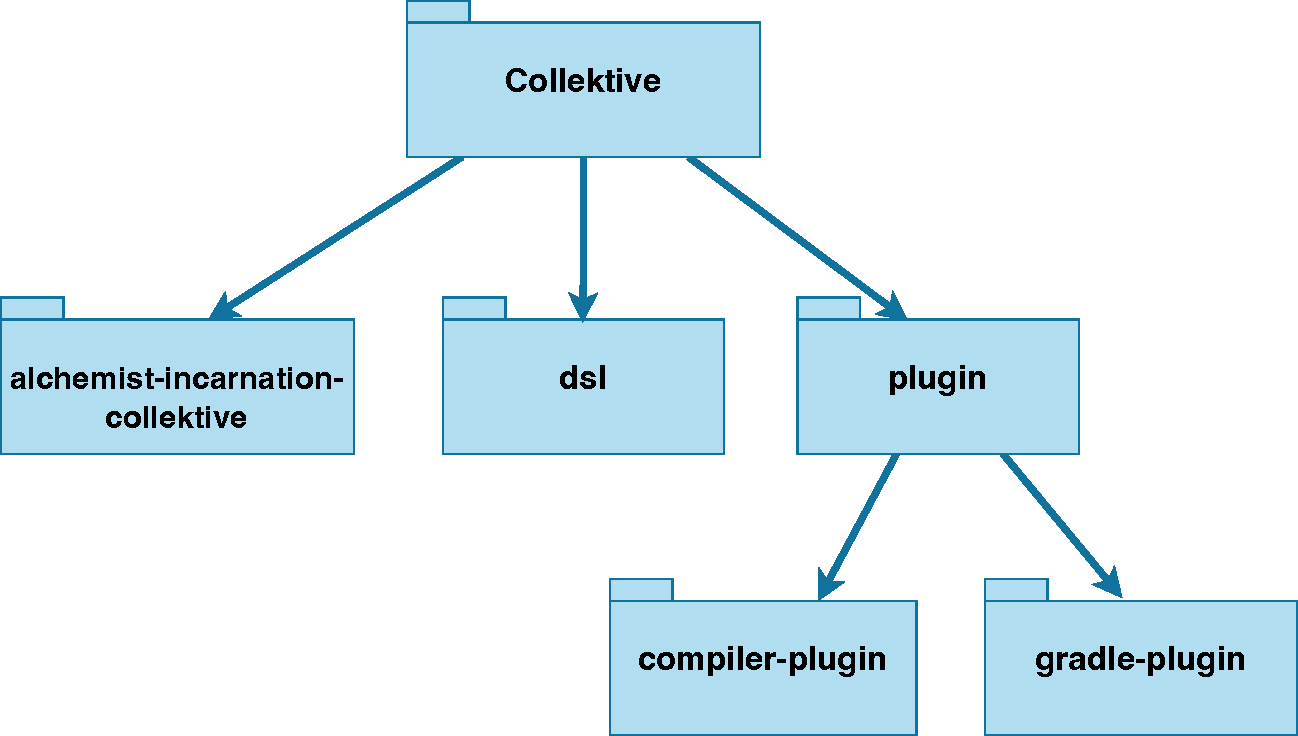
\includegraphics[width=0.7\textwidth]{figures/packages}
    \caption{Packages diagram of the Collektive project.}
    \label{fig:pacakges}
\end{figure}

Regarding the examples, there is a specific repository called \textbf{collektive-examples} that contains some samples of
aggregate programs to show how to use the \emph{Collektive} framework.

\section{DSL}
\label{sec:dsl}

In this thesis, the original implementation of the \ac{dsl} of \emph{Collektive} will be modified to allow the use of \xc{}
and to improve its performance.

A \ac{dsl} is a specialised programming language or language framework tailored to address the
requirements of a specific domain or problem area.
In contrast to general-purpose programming languages, which aim for versatility across various domains and problem categories,
DSLs are crafted to cater precisely to the demands of a particular application or system.
Consequently, general-purpose languages like Java typically exhibit greater complexity compared to \acp{dsl}.


\paragraph{Structure}
%todo add class diagrams
%For what it concerns the structure of the core of the project,
The \emph{Collektive}'s \ac{dsl} is composed of the following components:
\begin{itemize}
    \item \textbf{Path}: represents a specific point in the \ac{ast} of an aggregate program;
    \item \textbf{State}: is an association between a path and a value, it is used by the compiler plugin to
        keep track of the computational state of the device in order to provide the correct alignment of the nodes;
    \item \textbf{Field}: represents the \emph{computational field} used by aggregate constructs.
        It is a map of messages where the key is the identifier (ID) of the node, and the value is the associated message;
    \item \textbf{Message}: is an interface that represents the message exchanged between nodes, its concept will be explained in \ref{subsec:messages};
    \item \textbf{Network}: is the interface that represents the network used to manage the communication between devices;
    \item \textbf{Aggregate}: the actual core of the \ac{dsl}.
        It is also used to handle all the data needed for the computation; for example, the \emph{localId} and the \emph{state} of the device.
        It contains the primary functions on which the language is extended, such as \texttt{exchange}, \texttt{exchanging}, \texttt{repeat} and \texttt{repeating};
        To create an aggregate program, a function must extend this interface, in this way it will be possible to use the aggregate functions.
        It is also implemented the mechanism to handle the alignment of the functions used within the compiler plugin;
    \item \textbf{AggregateOperators}: contains the implementation of the functions created using the \texttt{exchange-exchanging} functions,
        such as \texttt{share}, \texttt{sharing} and \texttt{neighboringViaExchange}.
        Moreover, it contains the mechanism to manage the alignment of the fields used within the compiler plugin;
    \item \textbf{YieldSupport}: contains the \emph{Yielding Context} and the \emph{Yielding Result} for the ``yielding''
        operations, which means that the function operates on an initial value but possibly returns a different value;
    \item \textbf{Collektive}: is the entrypoint for creating a ``Collektive'' device, it must have a specific \emph{ID} and a
        \emph{network} to manage the communication between devices.
        The effective aggregate program is identified by the \emph{compute function}, which will be executed
    \item \textbf{AggregateResult}: is the result of one evaluation of the aggregate program, it contains the \emph{localId}
        of the node, the effective \emph{result} of the computation, the \emph{messages to send} to other devices and the \emph{new state} of the device;
\end{itemize}

\subsection{XC in Collektive}
\label{subsec:exchange-in-collektive}

Thanks to the design of \xc{}, it is possible to implement the methods proposed by \emph{field calculus}
(~\ref{par:syntax-of-field-calculus}) in terms of \emph{exchange} (~\ref{par:communication-in-xc}).
The syntax of \emph{XC} allows for sending messages to specific nodes, enabling the implementation of \emph{field calculus}
operations through message exchange.

The \emph{exchange} communication is based on \emph{anisotropic} communications, meaning that it has not the same properties
or characteristics in all directions (\Cref{fig:anisotropic}); therefore, messages have custom values sent to different neighbours.

\begin{figure}[h!]
    \centering
    \includegraphics[width=0.2\textwidth]{figures/anisotropic}
    \caption{Anisotropic communication.}
    \label{fig:anisotropic}
\end{figure}

This concept can be extended to the \texttt{share} function of field calculus, with the difference that the
operation of \texttt{share} is based on \emph{isotropic} communication, meaning that properties are uniform in all directions
(\Cref{fig:isotropic}); therefore, messages have the same value sent to all neighbours.

\begin{figure}[h!]
    \centering
    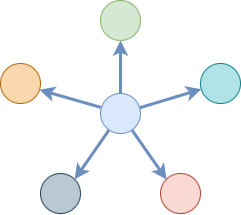
\includegraphics[width=0.2\textwidth]{figures/isotropic}
    \caption{Isotropic communication.}
    \label{fig:isotropic}
\end{figure}

All the \ac{dsl} has been modified to use \texttt{exchange} for the implementation of the other constructs such as \texttt{share}
and \texttt{nbr}, which is called \texttt{neighboring}.
Only the \texttt{rep} construct has not been implemented in terms of \texttt{exchange}, as it is a function that allows iterating
over oneself, it's better for neighbours not to receive messages of any kind, also for security and privacy reasons.
As the original implementation, it supports the evaluation of \emph{fields}.

\paragraph{Exchange}
The construct \texttt{exchange} provides
    \emph{(i)} access to neighbours' values,
    \emph{(ii)} persistence of information for subsequent executions,
    \emph{(iii)} communication with neighbours, and
    \emph{(iv)} compositional behaviour.

As seen in \ref{par:communication-in-xc}, the \texttt{exchange} function can send and return the same result, or it
can send a message and return a different result; both cases have been implemented.

%todo check that I say that the return is a field
%todo diagrams?

The \texttt{exchange} takes an \emph{initial} value to use as a default, and a \emph{body} that defines an aggregate
function to be computed, as seen in the code snippet \ref{lst:exchange}, returning a \emph{field}.
When executing the aggregate program, it checks which messages have been received from the neighbours and applies the function,
generating a custom value for each neighbour.

In the early stages of the design of this function, potential problems that could arise during execution were evaluated,
such as the management of initialisation, i.e.\ the first round of message exchange.
Consider a network consisting of $n$ devices, in which all are considered as neighbours to each other.
The first device ($d_1$) to start within the network will certainly have a moment when it performs its first iteration ever.

The problem arises when the device $d_1$ has not yet received any messages, so it will not have neighbour values to perform
the calculation, thus creating a deadlock situation where it does not know the neighbourhood and does not know who to actually send a message to.
For this reason, it was necessary to implement a mechanism such that the device performs a first iteration on its initial value,
and send the message to the network without a specific recipient, so that the future ``neighbourhood'' can receive it and start a communication with $d_1$.
In this way, the next devices to ``wake up'' in the network will know that $d_1$ is present and will be able to communicate with it.

\begin{lstlisting}[language=kt,label={lst:exchange}, caption={The signature of the \texttt{exchange} function.}]
fun <Initial> exchange(
    initial: Initial,
    body: (Field<ID, Initial>) -> Field<ID, Initial>,
): Field<ID, Initial>
\end{lstlisting}

\paragraph{Share}
The \texttt{share} construct captures the space-time nature of field computation through observation of neighbours' values,
starting from an \emph{initial} value, it reduces to a single local value given a \emph{transform} function and updating and sharing to
neighbours of a local variable, then returns the punctual value evaluated from the transformation (\ref{lst:share}).

\begin{lstlisting}[language=kt,label={lst:share}, caption={The signature of the \texttt{share} function.}]
fun <ID : Any, Initial> Aggregate<ID>.share(
    initial: Initial,
    transform: (Field<ID, Initial>) -> Initial,
): Initial
\end{lstlisting}

As previously introduced, this construct can be expressed in terms of \texttt{exchange}.
What \texttt{share} differs from it is that \texttt{share} does not differentiate the result of the computation based on
the neighbour that sent the message; it sends it indiscriminately to all neighbours.

\paragraph{Neighboring}

The \emph{field calculus} construct \texttt{nbr} is implemented as \texttt{neighboring}, more precisely as \texttt{neighboringViaExchange}
due to its effective implementation based on the \texttt{exchanging} function.
The \texttt{neighboringViaExchange} construct is used to access the values of the neighbours.
It takes as parameter \emph{local} (\ref{lst:neighboring}), which can be an expression or a value, and returns a \emph{field} of the same type.

\begin{lstlisting}[language=kt,label={lst:neighboring}, caption={The signature of the \texttt{neighboringViaExchange} function.}]
fun <ID : Any, Scalar> Aggregate<ID>.neighboringViaExchange(
    local: Scalar,
): Field<ID, Scalar>
\end{lstlisting}

%todo add something else???

\paragraph{Repeat}
The \texttt{repeat} function is the equivalent of the \texttt{rep} construct in \emph{field calculus}.
It models the state evolution over time, the value of \emph{initial} evolves at each execution depending on the \emph{transform} function,
and it returns the final value of the computation (\ref{lst:repeat}).

\begin{lstlisting}[language=kt,label={lst:repeat}, caption={The signature of the \texttt{repeat} function.}]
fun <Initial> repeat(
    initial: Initial,
    transform: (Initial) -> Initial,
): Initial
\end{lstlisting}

As previously mentioned, this function is not implemented in terms of \texttt{exchange}, because iterating over oneself
it is better not to send messages to neighbours, also for security and privacy reasons.

\subsection{Messages}
\label{subsec:messages}
%todo message modelling (in scafi there is an action that computes the messages and then creates a reaction that
%sends the message) we do it in a different way

The accurate modelling of message functionality is crucial for device communication.
Due to the different nature of messages supported, that is \emph{anisotropic} and \emph{isotropic} communication,
it has been necessary to create specific data classes for the handling of relative messages.

Previously, messages were sent to the network without considering the recipient, and the network was responsible for
delivering the message to all the neighbours that were interconnected.
Since the main feature of \texttt{exchange} is to send messages to specific neighbours with custom values, it is important
to ensure that unintended recipients do not receive the message.
Therefore, the old model of messages has been modified.

\paragraph{OutboundMessage and SingleOutboundMessage}
It has been introduced the concept of \emph{OutboundMessage} (\Cref{lst:outbound}), which is a data class that keeps track of the sender of the
message (its ID), and a map of messages, where the key is the \emph{Path} of the computation and the value is another data
class: the \emph{SingleOutboundMessage} (\Cref{lst:single}).
In this way, a device sends to the network just one \emph{OutboundMessage} that contains all the messages to send to the neighbours,
and also unburdens the payload of the network.

\begin{lstlisting}[language=kt,label={lst:outbound}, caption={Outbound message data class.}]
data class OutboundMessage<ID : Any>(
    val senderId: ID,
    val messages: Map<Path, SingleOutboundMessage<ID, *>>,
) : Message
\end{lstlisting}

\begin{lstlisting}[language=kt,label={lst:single}, caption={Single outbound message data class.}]
data class SingleOutboundMessage<ID : Any, Payload>(
    val default: Payload,
    val overrides: Map<ID, Payload>,
)
\end{lstlisting}

The main difference for the type of the communication lies in the \emph{SingleOutboundMessage} data class.
For what it concerns the \emph{anisotropic} communication, it is necessary to keep track of the identifier of the recipient
and the value associated with it, in order for the network to deliver the message to the correct neighbour.
This has been implemented with a map of \emph{overrides}, which associates to the recipient's identifier a specific value.

For the \emph{isotropic} communication, the \emph{SingleOutboundMessage} has a \emph{default} value, which is used
when there are no overrides for the recipient that is reading the messages received.

In summary, when a program is executed and a device has computed its function, it has to generate the messages to send to
the neighbours (so it's done inside the \texttt{exchange} function), it populates a \emph{SingleOutboundMessage},
that will be added to a list of \emph{OutboundMessage} and sent to the network.

\paragraph{InboundMessage}
The \emph{InboundMessage} is a data class (\Cref{lst:inbound}) modelled for the messages read from the network.
When reading the \emph{OutboundMessage}, there are some fields that are not needed, such as the receiver of the message,
which is the device itself, and is necessary to keep the default value or the override value.
To handle this, the \emph{InboundMessage} has been modelled to keep only the identifier of the sender and
a map of messages of \emph{Path} and the associated value.

\begin{lstlisting}[language=kt,label={lst:inbound}, caption={Inbound message data class.}]
data class InboundMessage<ID : Any>(
    val senderId: ID,
    val messages: Map<Path, *>,
) : Message
\end{lstlisting}

\subsection{Network}
\label{subsec:network}
The \emph{Network} has the task of managing only the reading and writing of messages in the network for a single device.
The actual implementation of the network is not managed by \emph{Collektive}, but it is the user's responsibility to manage
the network according to their needs.

%\subsectio%n{Syntax}
%\label{subsec:syntax}
%code
%rep non serve farla con xc perche non vogliamo che gli altri nodi ricevano il messaggio, cose che non gli interessano

\section{Plugin Extensions}
\label{sec:plugin-extensions}
In Kotlin, a plugin compiler extension refers to a mechanism that allows developers to extend or customise the behaviour
of the Kotlin compiler.
These extensions provide a way to hook into the compilation process and modify or enhance the way Kotlin code is compiled.

Developers can create their own compiler extensions by implementing the necessary interfaces or annotations defined by
the Kotlin compiler API.
These extensions can then be applied to Kotlin projects either globally or selectively, depending on the specific
requirements of the project.

\paragraph{Alignment}
%how
%todo

\section{Technologies}
\label{sec:technologies}
%multiplatform
%todo

\section{Implementation}
\label{sec:implementation}
%diagrams
%todo write something here
%dati i problemi e le scelte fatte, gli step di come è stata implementata l'exc sono i seguuenti e spiegare il codice


\subsection{Collektive entrypoint}
\label{subsec:collektive-entrypoint}
The public entrypoint of the \ac{dsl} is the \emph{Collektive} class, which can be interpreted as a device that can
execute an aggregate program.

As seen in the code snippet \ref{lst:collektive}, the \emph{Collektive} class takes as parameters the \emph{localId} of the device,
the \emph{network} used to manage the communication between devices, and the \emph{computeFunction} that will be executed
when the device is ready to compute the aggregate program.

\begin{lstlisting}[language=kt,label={lst:collektive}, caption={The signature of the \texttt{Collektive} class.}]
class Collektive<ID : Any, R>(
    val localId: ID,
    private val network: Network<ID>,
    private val computeFunction: Aggregate<ID>.() -> R,
)
\end{lstlisting}

The aim of this class is to manage the logic and the effective execution of the rounds of the aggregate program passed as a parameter.

It provides two main functions that will be called in the incarnation to execute the program:
\begin{itemize}
    \item \texttt{cycle}: applies once the \emph{computeFunction} and returns the result of the computation;
    \item \texttt{cycleWhile}: applies the \emph{computeFunction} while the condition passed as parameter is satisfied,
        and returns the result of the computation.
\end{itemize}

Both functions are implemented through a private function \texttt{executeRound}, which effectively calls the aggregate program,
managing the result obtained and updating the internal state of the device.

There are two types of aggregate programs: one that uses the \emph{Network} and one that does not, but directly takes
a set of \emph{InboundMessage}.

\begin{lstlisting}[language=kt,label={lst:aggregate}, caption={The signature of the \texttt{aggregate program}.}]
fun <ID : Any, R> aggregate(
        localId: ID,
        network: Network<ID>,
        previousState: State = emptyMap(),
        compute: Aggregate<ID>.() -> R,
    ): AggregateResult<ID, R> = with(AggregateContext(localId, network.read(), previousState)) {
        AggregateResult(localId, compute(), messagesToSend(), newState()).also {
            network.write(it.toSend)
        }
    }
\end{lstlisting}

The code seen in \ref{lst:aggregate} is the implementation of the \texttt{aggregate} function that relies on the \emph{Network}.
Taking the \emph{AggregateContext} as context with the messages read from the network and the previous state of the
device, it applies the \emph{compute} function.
The result of the computation is then returned as an \emph{AggregateResult} (\Cref{lst:aggregateresult}), which contains the \emph{localId} of the device,
the effective \emph{result} of the computation, the \emph{messages to send} to other devices and the \emph{new state} of the device.
Finally, the messages to send are written to the network.
This is the function called from the \texttt{executeRound} function.

\begin{lstlisting}[language=kt,label={lst:aggregateresult}, caption={The signature of the \texttt{aggregate result}.}]
data class AggregateResult<ID : Any, R>(
    val localId: ID,
    val result: R,
    val toSend: OutboundMessage<ID>,
    val newState: State,
)
\end{lstlisting}

\subsection{Yielding Support}
\label{subsec:yielding-support}
In order to make possible to operate on an initial value but possibly return a different value, it has been introduced
the concept of \emph{yielding}.
The operations of yielding are used to operate on an initial value, which is usually exchanged with the neighbours,
but possibly return a different value to the caller.
This operation is executable on the \texttt{exchanging}, \texttt{sharing} and \texttt{repeating} methods, or it can be omitted
in case the value obtained from the operation is to be returned. Those construct will be explained in detail in the
sections \ref{subsec:aggregate-context} and \ref{subsec:aggregate-operators}.

\begin{lstlisting}[language=kt,label={lst:yieldingcontext}, caption={The signature of the \texttt{yielding context} class.}]
class YieldingContext<Initial, Return> {
    fun Initial.yielding(toReturn: () -> Return): YieldingResult<Initial, Return> =
        YieldingResult(this, toReturn())
}
\end{lstlisting}

%todo explain the yielding thing


\subsection{Aggregate Context}
\label{subsec:aggregate-context}

The \emph{AggregateContext} class is the class that effectively has the implementation of the basic constructs inside the \ac{dsl}.
Internally, it keeps track of the {stack}, the state, and the messages that need to be sent by that device.

\paragraph{Exchange}
There are two versions of this construct: one that has the same type of value of the field in output as the one in input (\Cref{lst:exchangeImpl}),
and one in which they differ (\Cref{lst:exchanging}).
The \texttt{exchange} construct is the one that represents the communication in which $e_r$ (the value to return)
and $e_s$ (the value to send) coincide, as illustrated in \ref{par:communication-in-xc}.

\begin{lstlisting}[language=kt,label={lst:exchangeImpl},caption={The implementation of the \texttt{exchange} function.}]
fun <X> exchange(initial: X, body: (Field<ID, X>) -> Field<ID, X>): Field<ID, X> =
        exchanging(initial) { field -> body(field).run { yielding { this } } }
\end{lstlisting}

The \texttt{exchange} therefore simply calls the \texttt{exchanging}, but as the context of the yielding it passes the
field on which the computation has been executed.

The real functioning of \xc{} relies in the \texttt{exchanging} implementation, which is the one that effectively manages
the actual logic of the computation and the messages to send to the neighbours.

\begin{lstlisting}[language=kt,label={lst:exchanging},caption={The signature of the \texttt{exchanging} function.}]
fun <Initial, Return> exchanging(
        initial: Initial,
        body: YieldingScope<Field<ID, Initial>, Field<ID, Return>>,
    ): Field<ID, Return>
\end{lstlisting}

\subsection{Aggregate Operators}
\label{subsec:aggregate-operators}


\subsection{Using reflection}
\label{subsec:using-reflection}

%todo write the specific behaviour of the functions


\section{Alchemist Incarnation}
\label{sec:incarnation}
%how, why
%gradle task
%explain what is the alchemist incarnation
An ``incarnation'' serves as the interpreter enabling the \emph{Alchemist Simulator} to comprehend and accurately execute a language.
Specifically designed for \emph{Collektive}, this incarnation employs reflections to locate the aggregate entry point and dictates
the methodology for each iteration of the aggregate program.


%! Author = angela
%! Date = 24/01/24
% !TeX root = ../thesis-main.tex

\chapter{Contribution}
\label{chap:contribution}

You may also put some code snippet (which is NOT float by default), eg: \cref{lst:random-code}.

\lstinputlisting[float,language=Java,label={lst:random-code}]{listings/HelloWorld.java}

\section{Fancy formulas here}


%! Author = angela
%! Date = 24/01/24
% !TeX root = ../thesis-main.tex

\chapter{Conclusions}
\label{ch:conclusions}

\section{Future Works}
\label{sec:future-works}
%----------------------------------------------------------------------------------------
% BIBLIOGRAPHY
%----------------------------------------------------------------------------------------

\backmatter

\nocite{*} % comment this to only show the referenced entries from the .bib file

\bibliographystyle{alpha}
\bibliography{bibliography}


\begin{acknowledgements} % this is optional
    Benvenuti nell'unica sezione che molti di voi vorranno leggere, o per lo meno, in quella più facile da capire.
    Sì, non c'è di che, questa parte è in italiano.
    Parto chiedendo scudo perchè non sono molto sentimentale e faccio un po' schifo a scrivere queste cose, figuratevi
    se avessi scritto in inglese pure sta parte.
    Ma, in ogni caso, ci provo.

    Vorrei innanzitutto ringraziare il mio relatore, il Prof. Danilo Pianini, per avermi dato l'opportunità di lavorare
    a questo progetto e di unirmi al suo gruppo di ricerca.
    Un grande grazie anche a Nico (aka dottor correlatore), che mi ha sOpportata e aiutata durante tutto il percorso di tesi.

    Scrivere queste tre righe è stato veramente impegnativo.
    Ma comunque sia, ci tengo a ringraziare tutti i nuovi amichetti conosciuti durante quest'esperienza, dal \emph{Lab4.0} con
    Marti, Nico, Ange (il gioco), Magnus, Ruslan, Giovanni$^2$, al \emph{PsLab} con Gianlu, Dom e Samu, a tutti quelli
    di ``Disagio in 4.0++''.
    Grazie anche per tutte le risate fatte allo Shtop e alle varie serate assieme.

    Grazie anche alle \emph{Ragatte} e agli amiconi di una vita di Riolo: Arlessia, Smeo, Bananna, Sarabb, Diego, Rava, Fronz,
    Cri, Dave, Maicolle, Pulti e Santa; perdonate la mia trasformazione fantasma in questi ultimi mesi, rimedieremo asap.

    Non ringrazio gli ``Angeli'' (*'s Angels) perchè sono loro che devono ringraziare me per la mia presenza nella loro vita.
    Dai scherzo (ma se volete non scherzo), grazie per i pranzi, gli scleri, le boiate (e le collab nei progetti) a Leo,
    Angelo, Spaolo, Fosco, Eddie, Davide e Filo.
    Prego per gli stickers e per i photoshoppini, è stato un piacere.

    Grazie ai miei amiconi del \emph{Quesito scientifico di importanza fondante}, dobbiamo ancora trovare la risposta
    alla domanda, ma ci stiamo lavorando.

    Onorevol mention anche a tutti gli amici conosciuti durante gli anni dell'uni da \emph{inform-erda} a \emph{Notice me [...]},
    siete tanti e se vi nominassi tutti questa tesi diventerebbe un libro.
    Altra onorevol mention a tutti gli amiconi del Delta.

    Grazie a chi c'è sempre stato e a chi è stato solo di passaggio, siete stati tutti importanti.

    Ultimi ma non per importanza, ringrazio tutta la mia famiglia, che mi ha sempre supportata e lasciata libera di scegliere
    il mio percorso con fiducia.

    So che alcuni di voi si aspettavano qualche battuta "non convenzionale" (illegale), ma penso sia stato più faticoso
    scrivere questi ringraziamenti che la tesi stessa (sono in burnout totale scusate).
    Andate in pace.
\end{acknowledgements}

\end{document}